\chapter{Algoritmi probabilistici}
Il modello di calcolo di riferimento per gli algoritmi deterministici, inclusi quelli approssimanti visti fin'ora, è quello della macchina di Turing, in cui a un input corrisponde un output (\cref{fig:mdtdet}).
\begin{figure}[ht]
	\centering
	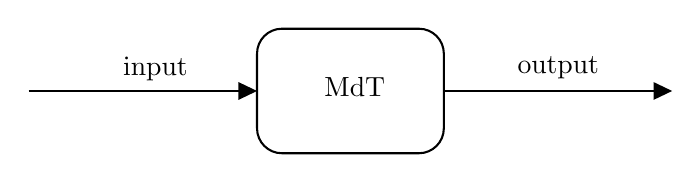
\begin{tikzpicture}[x=0.75pt,y=0.75pt,yscale=-1,xscale=1]
	\draw   (280,152) .. controls (280,145.37) and (285.37,140) .. (292,140) -- (358,140) .. controls (364.63,140) and (370,145.37) .. (370,152) -- (370,188) .. controls (370,194.63) and (364.63,200) .. (358,200) -- (292,200) .. controls (285.37,200) and (280,194.63) .. (280,188) -- cycle ;
	\draw    (170,170) -- (277,170) ;
	\draw [shift={(280,170)}, rotate = 180] [fill={rgb, 255:red, 0; green, 0; blue, 0 }  ][line width=0.08]  [draw opacity=0] (8.93,-4.29) -- (0,0) -- (8.93,4.29) -- cycle    ;
	\draw    (370,170) -- (477,170) ;
	\draw [shift={(480,170)}, rotate = 180] [fill={rgb, 255:red, 0; green, 0; blue, 0 }  ][line width=0.08]  [draw opacity=0] (8.93,-4.29) -- (0,0) -- (8.93,4.29) -- cycle    ;
	\draw (311,162) node [anchor=north west][inner sep=0.75pt]   [align=left] {MdT};
	\draw (214,152) node [anchor=north west][inner sep=0.75pt]   [align=left] {input};
	\draw (404,152) node [anchor=north west][inner sep=0.75pt]   [align=left] {output};
\end{tikzpicture}

	\caption{Macchina di Turing deterministica}
	\label{fig:mdtdet}
\end{figure}

Un diverso modello di calcolo è quello della macchina di Turing probabilistica (\cref{fig:mdtprob}), che ha accesso a una sorgente aleatoria, cioè un input secondario di bit casuali.

\begin{figure}[ht]
	\centering
	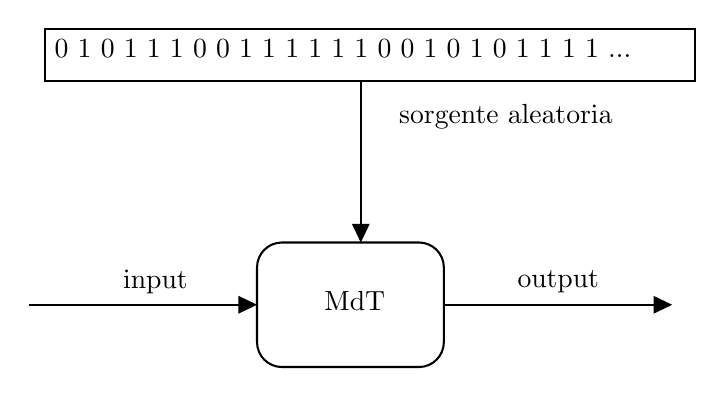
\begin{tikzpicture}[x=0.75pt,y=0.75pt,yscale=-1,xscale=1]
	\draw   (280,152) .. controls (280,145.37) and (285.37,140) .. (292,140) -- (358,140) .. controls (364.63,140) and (370,145.37) .. (370,152) -- (370,188) .. controls (370,194.63) and (364.63,200) .. (358,200) -- (292,200) .. controls (285.37,200) and (280,194.63) .. (280,188) -- cycle ;
	\draw    (170,170) -- (277,170) ;
	\draw [shift={(280,170)}, rotate = 180] [fill={rgb, 255:red, 0; green, 0; blue, 0 }  ][line width=0.08]  [draw opacity=0] (8.93,-4.29) -- (0,0) -- (8.93,4.29) -- cycle    ;
	\draw    (370,170) -- (477,170) ;
	\draw [shift={(480,170)}, rotate = 180] [fill={rgb, 255:red, 0; green, 0; blue, 0 }  ][line width=0.08]  [draw opacity=0] (8.93,-4.29) -- (0,0) -- (8.93,4.29) -- cycle    ;
	\draw    (330,62.29) -- (330,137) ;
	\draw [shift={(330,140)}, rotate = 270] [fill={rgb, 255:red, 0; green, 0; blue, 0 }  ][line width=0.08]  [draw opacity=0] (8.93,-4.29) -- (0,0) -- (8.93,4.29) -- cycle    ;
	\draw (311,162) node [anchor=north west][inner sep=0.75pt]   [align=left] {MdT};
	\draw (214,152) node [anchor=north west][inner sep=0.75pt]   [align=left] {input};
	\draw (404,152) node [anchor=north west][inner sep=0.75pt]   [align=left] {output};
	\draw (347,72) node [anchor=north west][inner sep=0.75pt]   [align=left] {sorgente aleatoria};
	\draw    (178,37) -- (491,37) -- (491,62) -- (178,62) -- cycle  ;
	\draw (181,41) node [anchor=north west][inner sep=0.75pt]   [align=left] { 0 1 0 1 1 1 0 0 1 1 1 1 1 1 0 0 1 0 1 0 1 1 1 1 ...};
\end{tikzpicture}

	\caption{Macchina di Turing probabilistica}
	\label{fig:mdtprob}
\end{figure}

Un algoritmo basato su questo modello si dice probabilistico, in quanto l'output dipende dall'input e dal seme casuale.
L'algoritmo possiede quindi una distribuzione associata, che mappa un input $x$ alla probabilità di ottenere l'output $y$:
\begin{equation*}
	P(Y = y \mid X = x)
\end{equation*}
Gli algoritmi probabilistici possono risolvere problemi di ottimizzazione quanto di decisione e si dividono in due famiglie:
\begin{description}
	\item[Monte Carlo] la correttezza dell'output, cioè la giusta decisione per i problemi di decisione e il calcolo della soluzione ottima per i problemi di ottimizzazione, è probabilistica; il tempo di esecuzione è deterministico;
	\item[Las Vegas] l'output è deterministicamente corretto; il tempo di esecuzione è probabilitico.
\end{description}
È possibile combinare algoritmi approssimanti con algoritmi probabilistici ottenendo algoritmi che approssimano entro una certa soglia dall'ottimo con una certa probabilità.



\section{\MinCut}
\MinCut è il problema di determinare il taglio minimo in un grafo non orientato. In un grafo non orientato $G=(V,E)$, un taglio è dato dalla partizione di $V$ in due sottoinsiemi $X, X\compl$. Il costo del taglio è dato dal numero di archi da vertici in $X$ a vertici in $X\compl$.
\popt{\MinCut}
{$G = (V,E)$}
{Taglio $X\subseteq V$}
{Determinare il taglio minimo in $G$}
{$X\subset V\mid X\neq\emptyset$}
{$\MIN$}
{$\card{\set{e\in E\mid e\cap X\neq\emptyset\land e\setminus X\neq\emptyset}}$}

\noindent\MinCut è un problema \NPO-completo.


\subsection{L'algoritmo di Karger}
L'algoritmo di Karger è un algoritmo Monte Carlo per il taglio minimo e si basa sull'operazione di contrazione.
Sia $G=(V,E)$ un multigrafo\footnote{Nei multigrafi sono ammessi lati paralleli, cioè più lati che incidono sulla stessa coppia di vertici. Consideriamo quindi $E$ un insieme dotato di molteplicità. Formalmente, all'insieme è associata una funzione che indica la molteplicità di ogni elemento. Useremo comunque per semplicità le nozioni insiemistiche per insiemi standard.} di input. Si consideri il multigrafo $G'=(V',E')$, dove:
\begin{itemize}
	\item $V':=\set{\bar v\mid v\in V}$, dove $\bar v:=\set{v}$;
	\item $E':=\set{\set{\bar u,\bar v}\mid \set{u,v}\in E}$.
\end{itemize}
La contrazione $G'\downarrow e$ del lato $e=\set{\bar u,\bar v}$ (\cref{fig:contrazione}) consiste in una modifica di $V'$ e $E'$ come segue:
\begin{enumerate}
	\item viene aggiunto a $V'$ un nuovo supervertice $\bar z=\bar u\cup\bar v$;
	\item ogni arco $\set{\bar u,\bar w}\in E'$, con $w\neq v$, è sostituito da un arco $\set{\bar z,\bar w}$;
	\item ogni arco $\set{\bar w,\bar v}\in E'$, con $w\neq u$, è sostituito da un arco $\set{\bar w,\bar z}$;
	\item gli archi del tipo $\set{\bar u,\bar v}$ vengono rimossi da $E'$;
	\item i vertici $\bar u,\bar v$ vengono rimossi da $V'$.
\end{enumerate}

% TODO: questa immagine andrebbe arricchita un po': non fa capire come si fondono gli archi
\begin{figure}[ht]
	\centering
	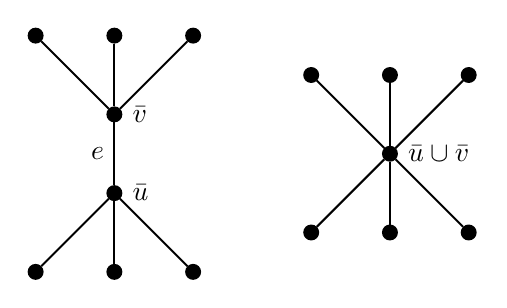
\begin{tikzpicture}[vertex/.style={draw,inner sep=0pt,minimum size=5pt,fill, circle}]
	\node[vertex] at (0, 2)  (u1) {};
	\node[vertex] at (-1, 2)  (u2) {};
	\node[vertex] at (1, 2)  (u3) {};
	\node[vertex,label={0:{$\bar u$}}] at (0, 0)  (a) {};
	\node[vertex,label={0:{$\bar v$}}] at (0, 1)  (b) {};
	\node[vertex] at (0, -1)  (l1) {};
	\node[vertex] at (-1, -1)  (l2) {};
	\node[vertex] at (1, -1)  (l3) {};
	\draw (u1) -- (b);
	\draw (u2) -- (b);
	\draw (u3) -- (b);
	\draw (l1) -- (a);
	\draw (l2) -- (a);
	\draw (l3) -- (a);
	\node at (1.75,0.5) (to) {$\implies$};
	\draw (a) edge node [left] {$e$} (b);
	\node[vertex] at (3.5, 1.5)  (lu1) {};
	\node[vertex] at (2.5, 1.5)  (lu2) {};
	\node[vertex] at (4.5, 1.5)  (lu3) {};
	\node[vertex,label={0:{$\bar u\cup \bar v$}}] at (3.5, 0.5)  (la) {};
	\node[vertex] at (3.5, -0.5)  (ll1) {};
	\node[vertex] at (2.5, -0.5)  (ll2) {};
	\node[vertex] at (4.5, -0.5)  (ll3) {};
	\draw (lu1) -- (la);
	\draw (lu2) -- (la);
	\draw (lu3) -- (la);
	\draw (ll1) -- (la);
	\draw (ll2) -- (la);
	\draw (ll3) -- (la);
\end{tikzpicture}

	\caption{Contrazione $G'\downarrow e$.}
	\label{fig:contrazione}
\end{figure}

In seguito chiameremo semplicemente $G$ il grafo $G'$ derivante dall'input. L'algoritmo \ref{algo:Karger} di Karger effettua contrazioni casuali a partire dal grafo $G$, ottenendo multigrafi $G_0,G_1,\dots$.

\begin{algorithm}[ht]
	\caption{Algoritmo di Karger per \MinCut}
	\label{algo:Karger}
	\SetKwFunction{Unif}{uniformExtraction}
	\SetKwFunction{Connected}{isConnected}
	\SetKwFunction{FindConnected}{findConnectedComponent}
	\SetKwFunction{Choose}{ChooseAnElement}
	\KwInput{grafo $G=(V,E)$}

	\If{$\lnot$\Connected{$G$}}{
		\Return{\FindConnected{$G$}}
	}
	\While{$\card V > 2$}{
		\tcp{Estrai uniformemente a caso un lato e contrailo}
		$e = \Unif{$E$}$

		$G = G\downarrow e$

	}
	\tcp{Restituisci uno dei due vertici rimanenti}
	\Return{\Choose{$V$}}
\end{algorithm}

Chiaramente, l'output dipende dalle scelte dei lati da contrarre, che sono casuali.
Sia $S\star$ il taglio minimo, $k\star$ il numero di lati tagliati da $S\star$ e $G_0,\dots,G_i,\dots$ la sequenza di grafi ottenuti per ogni contrazione operata dall'algoritmo, dove $G_i$ è ottenuto dopo $i$ passi. Si verificano i seguenti fatti:
\begin{oss}\label{oss:kargercontraction}
	\begin{equation*}
		\forall i \quad \card{V_i} = n-i \land \card{E_i} \leq m-i
	\end{equation*}
\end{oss}
\begin{oss}\label{oss:kargercuts}
	Per ogni $i$, ogni taglio in $G_i$ è un taglio in $G$ dello stesso costo.
\end{oss}
\begin{oss}\label{oss:kargermindeg}
	Il grado di ogni vertice di $G_i$ è maggiore o uguale a $k\star$.
\end{oss}

Proviamo ora due lemmi che ci serviranno per dimostrare che l'algoritmo di Karger ottiene la soluzione ottima con buona probabilità.
\begin{lemma}\label{lem:kargeredges}
	\begin{equation*}
		E_i \geq \frac{(n-i) \cdot k\star}{2}
	\end{equation*}
\end{lemma}
\begin{proof}
	\begin{align*}
		\sum_{v\in V_i} d_i(v) \geq \card{V_i} k\star \qquad & \text{per \cref{oss:kargermindeg}}      \\
		\sum_{v\in V_i} d_i(v) \geq (n-i) k\star  \qquad     & \text{per \cref{oss:kargercontraction}} \\
		% TODO: spiegare
		2\card{E_i} \geq (n-i) k\star                                                                  \\
		\card{E_i} \geq \frac{(n-i) k\star}{2}                                                         \\
	\end{align*}
\end{proof}

\begin{lemma}\label{lem:kargerprob_ei}
	Sia $E_i$ l'evento "al passo $i$-esimo (i.e. da $G_i$ a $G_{i+1}$) non viene contratto un lato del taglio minimo". Allora:
	\begin{equation*}
		\forall i \quad P(E_i \mid E_0, \dots, E_{i-1}) \geq \frac{n-i-2}{n-i}
	\end{equation*}
\end{lemma}
\begin{proof}
	\begin{align*}
		P(E_i \mid E_0,\dots,E_{i-1}) & = 1-P(\lnot E_i \mid E_0,\dots,E_{i -1})             \\
		                              & = 1-\frac{k\star}{\card{E_i}}                        \\
		                              & \geq 1-\frac{2k\star}{(n-i)k\star} = 1-\frac{2}{n-i} \\
		                              & = \frac{n-i-2}{n-i}
	\end{align*}
\end{proof}

\begin{theorem}
	L'algoritmo di Karger emette l'ottimo con probabilità $p \geq \frac{1}{{n\choose{2}}}$.
\end{theorem}
\begin{proof}
	L'algoritmo emette l'ottimo se non sono stati contratti archi nel taglio ottimo, ossia se si verifica l'evento $E_0\land E_1\land\dots\land E_{n-3}$. La probabilità di tale evento è
	\begin{align*}
		P(E_0\land E_1\land\dots\land E_{n-3}) & =P(E_0)\cdot P(E_1\mid E_0)\cdots P(E_{n-3}\mid E_0,\dots,E_{n-4})                                              \\
		                                       & \geq\frac{n-2}{n}\cdot\frac{n-3}{n-1}\cdots\frac{n-(n-3)-2}{n-(n-3)} \qquad \text{per \cref{lem:kargerprob_ei}} \\
		                                       & =\frac{n-2}{n}\cdot\frac{n-3}{n-1}\cdots\frac{1}{3}                                                             \\
		                                       & =\frac{(n-2)!}{n!/2}=\frac{2}{n(n-1)}=\frac{1}{\binom{n}{2}}
	\end{align*}
\end{proof}

\begin{corollario}
	Eseguendo l'algoritmo di Karger ${\binom{n}{2}}\ln n$ volte e scegliendo la migliore soluzione si ottiene l'ottimo con probabilità maggiore o uguale a $1-\frac{1}{n}$.
\end{corollario}
\begin{proof}
	Ad ogni esecuzione dell'algoritmo, la probabilità di non trovare l'ottimo è al più
	\begin{equation*}
		1-\frac{1}{\binom{n}{2}}\text.
	\end{equation*}
	Eseguendo l'algoritmo ${\binom{n}{2}}\ln n$ volte, la probabilità che nessun'esecuzione trovi l'ottimo è al più
	\begin{equation*}
		\left(1-\frac{1}{{\binom{n}{2}}}\right)^{{\binom{n}{2}}\ln n}\leq\left(\frac{1}{e}\right)^{\ln n}=\frac{1}{n}\text.
	\end{equation*}
\end{proof}

\section{Problema della copertura d'insiemi}
Abbiamo già definito il \textsc{SetCoverProblem}:
dato una serie di insiemi
$$
	S_1, \cdots, S_m \subseteq U
$$
con pesi
$$
	w_1 \cdots, w_m \in \mathbb{Q}^+
$$
definiamo $n = |U|$; vogliamo trovare un $S \subseteq m$ tale che
$$
	\bigcup_{i \in S} S_i = U
$$
e il suo costo $ \sum_{i \in S} w_i$ sia minimo.

\subsection{Algoritmo probabilistico basato sull'arrotondamento}
Il problema può essere trasposto in un problema di programmazione lineare intera:
creiamo delle variabili
$$
	x_1, \cdots, x_m
$$
tali che
$$
	\begin{cases}
		x_j \leq 1                     & \forall j = 1, \cdots, m \\
		x_j \geq 0                     & \forall j = 1, \cdots, m \\
		\sum_{i: u \in S_i} x_i \geq 1 & \forall u \in U
	\end{cases}
$$
Come sappiamo, i problemi di programmazione lineare intera appartengono alla
classe \textbf{NP-Completi}. Consideriamo dunque il problema $\Pi$ nella
sua versione non intera, $\Pi_{PL}$.

\`E importante richiamare ora alcune proprietà statistiche.
\begin{theorem}[Disuguaglianza di Markov]\label{thm:markov}
	Per ogni variabile aleatoria $X$ non negativa e per ogni $\alpha > 0$
	$$
		P[X \geq \alpha] \leq \frac{E[X]}{\alpha}
	$$
\end{theorem}

\begin{theorem}[Union bound o disuguaglianza di Boole]\label{thm:boole}
	$$
		P[\bigcup_{i} E_i] \leq \sum_i P[E_i]
	$$
\end{theorem}

\begin{algorithm}[h]
	\caption{\textsc{ProbabilisticRoundingSetCover}}
	\label{algo:ProbRoundingSetCover}
	\KwInput{$S_1, \cdots, S_m$, $w_1, \cdots, w_m$  e un intero $k$}

	$\hat{x_1}, \cdots, \hat{x_m} = solve(\Pi_{PL}) $

	$S =  \emptyset$

	\For {$t = \{1, \lceil k + \log(n) \rceil \}$}
	{

		\For {$i = 1, ..., m$}
		{
			\tcc*{Inserisci $i$ in $S$ con probabilità $\hat{x_i}$}
			$S = probInsert(S, i, \hat{x_i})$
		}
	}

	\Return {$S$}
\end{algorithm}

L'\cref{algo:ProbRoundingSetCover} potrebbe trovare una soluzione non ammissibile. Dimostriamo
ora che \textit{spesso} è ammissibile e che quando è ammissibile è una soluzione molto buona.

\begin{theorem}
	La probabilità che l'\cref{algo:ProbRoundingSetCover} produca una soluzione ammissibile è
	$$
		p \geq 1 - e ^ {-k}
	$$
	parametrica in $k$, che determina il numero di tentativi di inserimento.
\end{theorem}
\begin{proof}
	$$
		P[\text{soluzione ammissibile}] = 1 - P[\text{almeno un elemento dell'universo non è coperto}]
	$$
	chiamiamo $B_u$ l'evento per cui $u$ non è coperto nella soluzione. Allora
	$$
		P[\text{soluzione ammissibile}] = 1 - P[\bigcup_{u \in U} B_u]
	$$
	Possiamo quindi usare il \cref{thm:boole}:
	$$
		1 - P[\bigcup_{u \in U} B_u] \geq 1 - \sum_{u \in U} P[B_u]
	$$
	L'elemento $u$ non è coperto quando nessuno degli elementi che contentono
	$u$ non è stato scelto. Ad ogni iterazione, che sono
	$\lceil k + \log(n) \rceil$ in totale, ogni insieme ha probabilità
	$\hat{x_i}$ di essere scelto:
	\begin{align*}
		1 - \sum_{u \in U} \prod_{i: u \in S_i} P[S_i \text{ non è stato scelto}] & = 1 - \sum_{u \in U} \prod_{i: u \in S_i} (1 - \hat{x_i})^{\lceil k + \log(n) \rceil}	\\
		& \geq 1 - \sum_{u \in U} \prod_{i : u \in S_i} e^{-\hat{x_i} (k + \log(n))} & \text{nota che } 1 - x \leq e^{-x}													\\
		& = 1 - \sum_{u \in U} \exp(- (k + \log (n)) \sum_{i: u \in S_i} \hat{x_i})
	\end{align*}
	Siccome $S_i$ è ammissibile, deve essere $\sum_{i: u \in S_i} \hat{x_i}  \geq 1$, quindi
	\begin{align*}
		\geq 1 - \sum_{u \in U} e^{- (k + \log(n))} = 1 - \sum_{u \in U} \frac{e^{-k}}{n}  = 1 - e^{-k} \frac{1}{n}|U| = 1 - e^{-k}
	\end{align*}
\end{proof}

\begin{theorem} \label{thm:ProbRoundingSetCoveralpha}
	$$\forall \alpha  ~~ 0 \leq \alpha \leq 1 ~~ P[\frac{v_{out}}{v^*}\geq \alpha (k + \log(n))] \leq \frac{1}{\alpha}$$
\end{theorem}
\begin{proof}
	Abbiamo che $\hat{v} = \sum_{i} w_i \hat{x_I} \leq v^*$; inoltre,
	la probabilità che $S_i$ venga scelto è

	\begin{align*}
		P[ S_i \text{ sia scelto}] & = P[ \bigcup_{t} S_i \text{ sia scelto durante l'iterazione } t] 	\\
		& \leq \sum_t P[S_i \text{ sia scelto durante l'iterazione } t] & \text{per \cref{thm:boole}}	\\ 
		& = (k + \log (n))\hat{x}_i
	\end{align*}

	Per poter utilizzare il \cref{thm:markov} calcoliamo il valore atteso di $v_{out}$:
	\begin{align*}
		E[v_{out}] & = \sum_{i} w_i P[S_i \text{ sia scelto}] 							\\
		& \leq \sum_i w_i (k + \log(n)) \hat{x_i} & \text{per osservazione precedente} 	\\
		& = \hat{v} (k + \log(n)) & \text{ricorda che } \hat{v}=\sum_i w_i \hat{x_i} 	\\
		& \leq v^* (k + \log(n))
	\end{align*}

	Infine utilizziamo questa osservazione per determinare la probabilità che
	la nostra soluzione approssimi bene il problema:
	\begin{align*}
		P [ \frac{v_{out}}{v^*} \geq \alpha (k + \log(n))] & = P [ v_{out} \geq v^* \alpha (k + \log(n)) ] 	\\
		& \leq \frac{E[v_{out}]}{\alpha (k + \log(n))v^*} & \text{applico Markov} 							\\
		& \leq \frac{v^* (k + \log(n))}{\alpha (k + \log(n))v^*} & \text{applico l'osservazione precedente}	\\ 
		& = \frac{1}{\alpha}		
	\end{align*}
\end{proof}

\begin{oss}
	Se si esegue l'\cref{algo:ProbRoundingSetCover} con $k = 3$ c'è il $45\%$ di probabilità di ottenere
	una soluzione ammissibile con fattore di approssimazione $\frac{v_{out}}{v^*}\leq 6 + 2 \log (n)$.
\end{oss}
\begin{proof}
	Sia $E_{ammissibile}$ l'evento per cui si ottiene una soluzione ammissible e
	$E_{buona}$ l'evento per cui l'output sia entro $6 + 2 \log(n)$ dall'ottimo.
	Ci interessa
	\begin{align*}
		 & P[E_{ammissibile} \land E_{buona}] = 1 - P[\neg E_{ammissible} \lor
		\neg E_{buona}] \geq 1 - P[\neg E_{ammissibile}] - P[\neg E_{buona}]                                  \\
		 & \geq 1 - e^{-3} - \frac{1}{2} \approx 0.45  ~~~  (\text{dal \cref{thm:ProbRoundingSetCoveralpha}})
	\end{align*}
\end{proof}

\section{Problema MaxEkSat}
\textsc{MaxEkSat} è la versione $k$-indicizzata di \textsc{MaxSat}: date $t$ clausole
di $k$ letterali ciascuna, l'obiettivo è massimizzare il numero di clausole
soddisfatte.

Definiamo $x_1, \cdots, x_n$ le variabili che compaiono nella formula
e $c_1, \cdots, c_t$ le clausole della formula.

\begin{theorem}\label{thm:maxeksatnp}
	\textsc{MaxEkSat} $\in \mathbf{NPO-completi}$ per $k \leq 3$.
\end{theorem}

\subsection{Algoritmo probabilistico}
\begin{theorem}\label{thm:probassgn}
	Assegnando casualmente le variabili, il valore atteso di clausole soddisfatte è
	$$
		E[T] = \frac{2^k-1}{2^k} t
	$$
\end{theorem}
\begin{proof}
	Per la dimostrazione definiamo
	$$
		X_i \sim Unif(\{0,1\})
	$$
	il valore assegnato ad ogni $x_i$ probabilisticamente;
	$$
		C_i =
		\begin{cases}
			1 & C_i \text{ soddisfatto} \\
			0 & \text{ altrimenti}
		\end{cases}
	$$
	mentre $T=\sum_i^t C_i$ è il numero di clausole soddisfatte.
	L'algoritmo si svolge, banalmente, estraendo un valore per ogni $x_i$
	e restituendo il numero di clausole soddisfatte.

	\begin{oss}\label{oss:ciatteso}
		$$
			\forall i ~ \sum_{b_1 \in 2} \sum_{b_2 \in 2} \cdots \sum_{b_n \in 2} E[C_i | X_1=b_1 \cdots x_n=b_n] = 2^n - 2^{n - k}
		$$
	\end{oss}
	\begin{proof}
		Consideriamo una generica clausola $c_i$ e la sua variabile aleatoria
		associata $C_i$. Una volta che è stato fissato un assegnamento di
		valori di verità $b_1 \cdots b_n$, il valore di
		$E[C_i | X_1=b_1 \cdots x_n=b_n]$ sarà semplicemente $1$ o $0$, in base
		a se quell'assegnamento soddisfa la clausola $c_i$ o meno.

		Possiamo dunque vedere
		$$
			\sum_{b_1 \in 2} \sum_{b_2 \in 2} \cdots \sum_{b_n \in 2} E[C_i | X_1=b_1 \cdots x_n=b_n]
		$$
		semplicemente come il numero di assegnamenti che soddisfano la clausola
		$c_i$.
		Per contare questo numero, consideriamo che il valore di verità di una
		clausola dipende solamente dai valori delle $k$ variabili che contiene
		al suo interno, le altre $n-k$ variabili non sono importanti.
		Essendo questi $k$ letterali tutti in $\vee$ tra di loro, se uno di
		questi è \textit{True} allora l'intera clausola è soddisfatta.

		Vedendo questa osservazione all'opposto, per rendere la clausola falsa
		dobbiamo fissare le $k$ variabili con un assegnamento specifico per
		rendere tutti i loro letterali \textit{False}, e le rimanenti $n-k$
		variabili possono assumere qualunque valore. Da questo otteniamo
		che ci sono $2^{n-k}$ assegnamenti che \textit{non} soddisfano la
		clausola, dunque ne esistono $2^n - 2^{n-k}$ che la soddisfano.
	\end{proof}

	Prima di procedere con la dimostrazione, ricordiamo la seguente legge
	statistica:
	\begin{theorem}\label{thm:leggevat}
		Sia $\{\mathcal{E}_i\}_{i=1..k}$ una partizione dell'universo degli eventi.
		Allora
		$$
			E[X] = \sum_{i = 1}^{k} E[X|\mathcal{E}_i]P[\mathcal{E}_i]
		$$
	\end{theorem}

	La partizione $\{\mathcal{E}_i\}_i$ nel contesto di \textsc{MaxEkSat} è l'insieme
	dei possibili assegnamenti $X_1 = b_1, \cdots, X_n = b_n$; pertanto
	\begin{align*}
		E[T] & = \sum_{b_1 \in 2} \cdots \sum_{b_n\in 2} E[T|X_i = b_1, \cdots, X_n = b_n]P[X_1 = b_1, \cdots, X_n = b_n]   											\\
		     & = \sum_{b_1 \in 2} \cdots \sum_{b_n\in 2} E[T|X_i = b_1, \cdots, X_n = b_n]P[X_1 = b_1] \cdots P[X_n = b_n]  											\\
		     & = \frac{1}{2^n}\sum_{b_1 \in 2} \cdots \sum_{b_n\in 2} E[T|X_i = b_1, \cdots, X_n = b_n]                     											\\
			 & = \frac{1}{2^n}\sum_{b_1 \in 2} \cdots \sum_{b_n \in 2} E[C_1 + ... + C_t | X_i = b_1, \cdots, X_n = b_n] & \text{Per definizione di T}					\\
		     & = \frac{1}{2^n}\sum_{j = 1}^{t}(\sum_{b_1 \in 2} \cdots \sum_{b_n\in 2} E[C_j|X_i = b_1, \cdots, X_n = b_n]) & \text{Per linearità del valore atteso} 	\\
		     & = \frac{1}{2^n} \sum_{j = 1}^t (2^n - 2^{n -k}) = \frac{2^n - 2^{n-k}}{2^n}t & \text{Applico \cref{oss:ciatteso}} 										\\
			& = \frac{2^k - 1}{2^k}t
	\end{align*}
\end{proof}

\subsection{Algoritmo derandomizzato}
\begin{theorem}\label{thm:maxsatderandomexv}
	Per ogni $j  = 0, \cdots, n$ esistono $b_1, \cdots b_j \in 2$ tali che
	$$
		E[T|X_1 = b_1, \cdots, X_j = b_j] \geq \frac{2^k-1}{2^k}t
	$$
\end{theorem}
Questo significa che non solo il numero atteso di clausole è \textit{alto}, ma
possiamo inoltre fissare le prime $j$ variabili in modo che questa proprietà
continui ad essere preservata.
\begin{proof}
	Per induzione su $j$.
	Il caso base $j = 0$ è verificato dal \cref{thm:probassgn}.
	Nel passo induttivo partiamo dall'ipotesi
	$$
		E[T|X_1 = b_1, \cdots, X_j = b_j] \geq \frac{2^k-1}{2^k}t
	$$
	Per il \cref{thm:leggevat} vale
	\begin{align*}
		&E[T|X_1 = b_1, \cdots, X_j = b_j] = \\
		&= E[T | X_1 = b_1, \cdots X_j = b_j, X_{j+1} = 0] P[X_{j+1} = 0] + E[T | X_1 = b_1, \cdots X_j = b_j, X_{j+1} = 1]P[X_{j+1} = 1]	\\
		&= \frac{1}{2} E[T | X_1 = b_1, \cdots X_j = b_j, X_{j+1} = 0] + \frac{1}{2} E[T | X_1 = b_1, \cdots X_j = b_j, X_{j+1} = 1]		\\
		&= \frac{1}{2} \alpha_0 + \frac{1}{2} \alpha_1
	\end{align*}
	Per assurdo, supponiamo che entrambi $\alpha_0$ e $\alpha_1$ siano
	strettamente minori di $\frac{2^k-1}{2^k}t$: allora
	$$
		E[T|X_1 = b_1, \cdots, X_j = b_j] = \frac{1}{2} \alpha_0 + \frac{1}{2} \alpha_1 < \frac{1}{2}\frac{2^k -1 }{2^k} t + \frac{1}{2} \frac{2^k -1 }{2^k} t = \frac{2^k -1 }{2^k} t
	$$
	ma questo contraddice l'ipotesi induttiva, concludiamo dunque che almeno
	uno tra $\alpha_0$ e $\alpha_1$ è $\geq \frac{2^k-1}{2^k}t$, soddisfacendo
	il passo induttivo.
\end{proof}

\begin{algorithm}[h]
	\caption{\textsc{DerandomMaxEkSat}}
	\label{algo:DerandomMaxEkSat}

	$D = \emptyset$ \tcp*{indici delle clausole già determinate}

	\For{$i = 1,\cdots, n$}
	{
		$\Delta_0 = 0$

		$\Delta_1 = 0$

		$\Delta D_0 = \emptyset$

		$\Delta D_1 = \emptyset$

		\For {$ j = 1, \cdots, t$}
		{
			\If{$ j \in D$}
			{
				\textbf{continue}
			}
			\If { $x_i \notin c_j$}
			{
				\textbf{continue}
			}

			$h = |\{x_k | k \geq i \land (x_k \in c_j \lor \neg x_k \in c_j)\}|$ \tcp*{num variabili con indice $\geq i$ in $c_j$}

			\If {$x_i$ non compare negata in $c_j$}
			{

				$\Delta_0 = \Delta_0 - \frac{1}{2^h}$

				$\Delta_1 = \Delta_1 + \frac{1}{2^h}$

				$\Delta D_1 = \Delta D_1 \cup \{j\}$

			} \Else {
				$\Delta_0 = \Delta_0 + \frac{1}{2^h}$

				$\Delta_1 = \Delta_1 - \frac{1}{2^h}$

				$\Delta D_0 = \Delta D_0 \cup \{j\}$

			}

		}

		$ u = \arg \max_{0,1} \{\Delta_0, \Delta_1\}$

		$x_i = u$

		$D = D \cup \Delta D_u$
	}
\end{algorithm}
L'idea di questo algoritmo è quella di assegnare le variabili passo per passo
in modo tale da far valere sempre
$$
	E[T|X_1 = x_1, \cdots, X_i = x_i] \geq \frac{2^k-1}{2^k}t
$$
A tal proposito ad ogni iterazione del ciclo più esterno vengono calcolati due
valori $\Delta_0$ e $\Delta_1$ che rappresentano la differenza tra il valore
atteso attuale e quello che si otterrebbe fissando la variabile $x_i$
rispettivamente a $0$ oppure a $1$.

Alla fine di ogni ciclo sceglieremo sempre di assegnare ad $x_i$ il valore
con il rispettivo $\Delta$ maggiore tra i due, in modo tale da mantenere
$E[T|X_1 = x_1, \cdots, X_i = x_i]$ sempre sopra la soglia.

Analizziamo ora il calcolo di $\Delta_0$ e $\Delta_1$.
Ricordiamo per prima cosa che
$$
	E[T|X_1 = x_1, \cdots] = E[C_1 + \cdots + C_t | X_1=x_1, \cdots] = E[C_1 | X_1=x_1, \cdots] + \cdots + E[C_t | X_1=x_1, \cdots]
$$
In un determinato momento ogni $E[C_j | X_1=x_1, \cdots, X_i=x_i]$ può trovarsi
in una di due situazioni: potrebbe avere un valore costante $0$ o $1$ perchè la
clausola $c_j$ è ormai determinata; in questa situazione il valore atteso non
potrà più cambiare in futuro dunque possiamo trascurarla nel calcolo delle
differenze.

Il secondo caso è quello in cui il valore atteso ha un valore dipendente dal
numero $h$ di variabili non ancora assegnate nella clausola. Questo valore
sarà $\frac{2^h - 1}{2^h}$ (perchè esiste un solo assegnamento che può
falsificare la clausola).
Osservando i possibili modi in cui può cambiare il valore atteso quando
assegniamo una variabile $x_i$ possiamo scoprire che la differenza tra
il valore atteso prima di assegnare $x_i$ e dopo averlo assegnato è sempre
$\frac{1}{2^h}$.
\begin{itemize}
	\item Se assegnando $x_i$ la clausola viene soddisfatta allora il valore
	atteso $E[T|X_1 = x_1, \cdots X_i=x_i] = 1$. In questa situazione
	$$
		1 - \frac{2^h - 1}{2^h} = \frac{2^h - 2^h + 1}{2^h} = \frac{1}{2^h}
	$$

	\item Se assegnando $x_i$ la clausola viene definitivamente falsificata,
	dunque non contiene più variabili libere, allora il valore atteso
	$E[T|X_1 = x_1, \cdots X_i=x_i] = 0$ e $h=1$, dunque
	$$
		\frac{2^h - 1}{2^h} - 0 = \frac{2^h - 1}{2^h} = \frac{1}{2^h}
	$$

	\item Se assegnando $x_i$ la clausola è ancora indeterminata allora
	la differenza tra i valori attesi prima e dopo l'assegnamento è
	$$
		\frac{2^h - 1}{2^h} - \frac{2^{h-1} - 1}{2^{h-1}} = \frac{2^h - 1 - 2^h + 2}{2^h} = \frac{1}{2^h}
	$$
\end{itemize}

\begin{theorem}
	L'\cref{algo:DerandomMaxEkSat} trova un assegnamento che soddisfa
	$$
		\geq \frac{2^k -1}{2^k} t
	$$
	clausole.
\end{theorem}
\begin{proof}
	Abbiamo dimostrato che l'algoritmo mantiene valido il
	\cref{thm:maxsatderandomexv} ad ogni iterazione, dunque anche all'ultima.
\end{proof}
\begin{corollario}
	L'\cref{algo:DerandomMaxEkSat} fornisce una $\frac{2^k}{2^k -1}$-approssimazione per
	\textsc{MaxEkSat}.
\end{corollario}
\begin{proof}
	Sia $t^*$ il numero ottimo di clausole soddisfatte. Si ha ovviamente $t^* \leq t$.
	Abbiamo, allora
	$$
		\frac{t^*}{t_{algo}} \leq \frac{t}{t_{algo}} \leq \frac{t}{\frac{2^k -1}{2^k} t}  = \frac{2^k}{2^k -1}.
	$$
\end{proof}

\section{Il teorema PCP}
Un punto fondamentale nell'analisi degli algoritmi proposta in questo corso sarà
l'analisi dell'inapprossimabilità di alcuni problemi. Per poter analizzare la questione
sarà necessario introdurre uno dei più importanti teoremi della teoria della complessità
dal teorema di Cook: il teorema PCP, \textit{probabilistically checkable proofs}.
Il punto di partenza per arrivare all'enunciato di PCP è descrivere un'estensione delle
macchine di Turing deterministiche.

\subsection{Macchine di Turing oracolari}
Le MdT oracolari ricevono in input un certo $x \in 2^*$ e in output restituiscono
un valore booleano, una risposta $True$ o $False$ per un certo problema di decisione.
Queste MdT hanno però anche accesso ad una \textit{stringa} o
\textit{nastro dell'oracolo} $w \in 2^*$;
se vuole accedere alla stringa dell'oracolo, la MdT ha un nastro speciale,
definito \textit{nastro di query} sul quale all'occorrenza può scrivere un numero
binario; una volta scritto tale numero, la macchina entra in uno stato speciale
che ``aspetta'' la risposta dell'oracolo: la MdT userà il numero scritto sul nastro
di query come posizione in cui leggere $w$, che conterrà un $1$ o uno $0$.
La MdT passerà ad uno stato relativo al numero trovato in $w$:
$$
	\text{stato speciale di interrogazione: } q?
	\begin{cases}
		w[n] = 1 & \rightarrow q_1 \\
		w[n] = 0 & \rightarrow q_0
	\end{cases}
$$
\begin{figure}[h]
	\begin{center}
		\tikzset{every picture/.style={line width=0.75pt}} %set default line width to 0.75pt        

		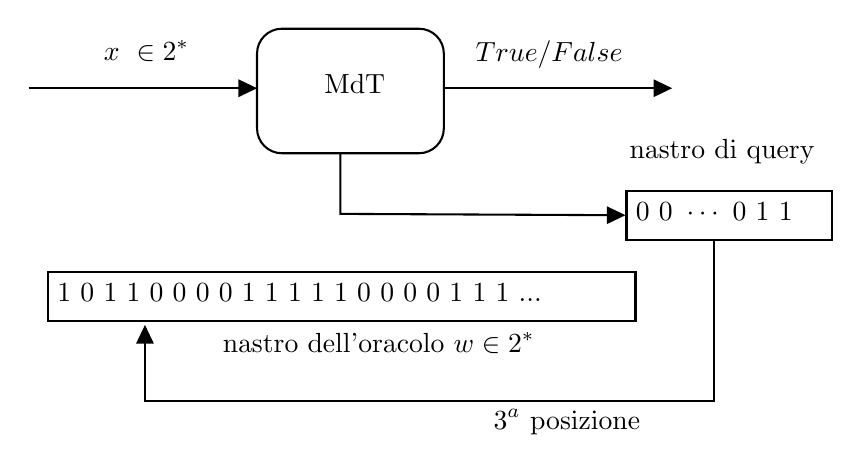
\begin{tikzpicture}[x=0.75pt,y=0.75pt,yscale=-1,xscale=1]
			%uncomment if require: \path (0,437); %set diagram left start at 0, and has height of 437

			%Rounded Rect [id:dp7665142760923608] 
			\draw   (280,152) .. controls (280,145.37) and (285.37,140) .. (292,140) -- (358,140) .. controls (364.63,140) and (370,145.37) .. (370,152) -- (370,188) .. controls (370,194.63) and (364.63,200) .. (358,200) -- (292,200) .. controls (285.37,200) and (280,194.63) .. (280,188) -- cycle ;
			%Straight Lines [id:da12014265713573546] 
			\draw    (170,168.67) -- (277,168.67) ;
			\draw [shift={(280,168.67)}, rotate = 180] [fill={rgb, 255:red, 0; green, 0; blue, 0 }  ][line width=0.08]  [draw opacity=0] (8.93,-4.29) -- (0,0) -- (8.93,4.29) -- cycle    ;
			%Straight Lines [id:da500409813700509] 
			\draw    (370,168.67) -- (477,168.67) ;
			\draw [shift={(480,168.67)}, rotate = 180] [fill={rgb, 255:red, 0; green, 0; blue, 0 }  ][line width=0.08]  [draw opacity=0] (8.93,-4.29) -- (0,0) -- (8.93,4.29) -- cycle    ;
			%Straight Lines [id:da6813515968969535] 
			\draw    (320.13,199.88) -- (320.13,214.71) -- (320.13,229.21) -- (454.13,229.85) -- (454.5,229.85) ;
			\draw [shift={(457.5,229.85)}, rotate = 180] [fill={rgb, 255:red, 0; green, 0; blue, 0 }  ][line width=0.08]  [draw opacity=0] (8.93,-4.29) -- (0,0) -- (8.93,4.29) -- cycle    ;
			%Straight Lines [id:da0793943852727933] 
			\draw    (500,242.31) -- (500,319.25) -- (226,319.25) -- (226,285.75) ;
			\draw [shift={(226,282.75)}, rotate = 90] [fill={rgb, 255:red, 0; green, 0; blue, 0 }  ][line width=0.08]  [draw opacity=0] (8.93,-4.29) -- (0,0) -- (8.93,4.29) -- cycle    ;

			% Text Node
			\draw (311,160.67) node [anchor=north west][inner sep=0.75pt]   [align=left] {MdT};
			% Text Node
			\draw (204.67,144) node [anchor=north west][inner sep=0.75pt]   [align=left] {$\displaystyle x\ \in 2^{*}$};
			% Text Node
			\draw (383.83,144.5) node [anchor=north west][inner sep=0.75pt]   [align=left] {$\displaystyle True/False$};
			% Text Node
			\draw    (179.33,257) -- (462.33,257) -- (462.33,281) -- (179.33,281) -- cycle  ;
			\draw (182.33,261.4) node [anchor=north west][inner sep=0.75pt]    {$1\ 0\ 1\ 1\ 0\ 0\ 0\ 0\ 1\ 1\ 1\ 1\ 1\ 0\ 0\ 0\ 0\ 1\ 1\ 1\ ...\ $};
			% Text Node
			\draw (262,284.83) node [anchor=north west][inner sep=0.75pt]   [align=left] {nastro dell'oracolo $\displaystyle w\in 2^{*}$};
			% Text Node
			\draw    (458,218) -- (557,218) -- (557,242) -- (458,242) -- cycle  ;
			\draw (461,222.4) node [anchor=north west][inner sep=0.75pt]    {$0\ 0\ \cdots \ 0\ 1\ 1$};
			% Text Node
			\draw (458,192) node [anchor=north west][inner sep=0.75pt]   [align=left] {nastro di query};
			% Text Node
			\draw (392.5,322) node [anchor=north west][inner sep=0.75pt]   [align=left] {$\displaystyle 3^{a}$ posizione};


		\end{tikzpicture}

	\end{center}
	\caption{La MdT è dotata di un nastro di query sulla quale scrive un numero quando necessario e, in base al numero scritto, accede al nastro dell'oracolo.}
	\label{fig:mdtoracle}
\end{figure}

Le MdT con oracolo sono il modo moderno per definire le classi nondeterministiche di macchine
di Turing.

\begin{theorem}
	Un linguaggio binario $L \subseteq 2^*$ appartiene a $\mathbf{NP}$ se e solo
	se esiste una MdT oracolare $v$ tale che:
	\begin{itemize}
		\item $v(x,w)$ termina in un numero polinomiale nella lunghezza $|x|$; e
		\item $\forall x \in 2^* ~ \exists w \in 2^* : v(w,x) = True$
		      se e solo se $x \in L$.
	\end{itemize}
\end{theorem}

\subsection{Probabilistic checkers}
Un'estensione delle MdT oracolari sono i \textit{probablistic checkers}:
anch'essi hanno accesso ad un oracolo e, in più, possono accedere ad una
\textit{sorgente di bit casuali} forniti su un nastro apposito. Nuovamente,
questo verificatore emetterà un valore tra $True$ e $False$; il suo comportamento,
ovviamente, dipenderà da $x$, $w$, e $r \in 2^*$, la stringa casuale.
\begin{figure}[h]
	\begin{center}
		\tikzset{every picture/.style={line width=0.75pt}} %set default line width to 0.75pt        

		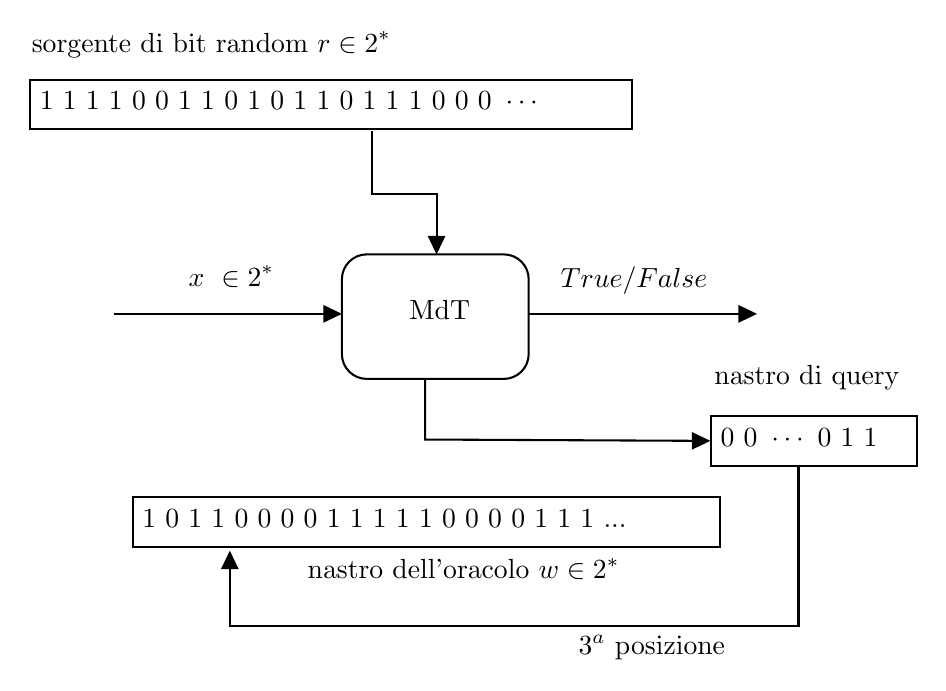
\begin{tikzpicture}[x=0.75pt,y=0.75pt,yscale=-1,xscale=1]
			%uncomment if require: \path (0,437); %set diagram left start at 0, and has height of 437

			%Rounded Rect [id:dp7665142760923608] 
			\draw   (280,152) .. controls (280,145.37) and (285.37,140) .. (292,140) -- (358,140) .. controls (364.63,140) and (370,145.37) .. (370,152) -- (370,188) .. controls (370,194.63) and (364.63,200) .. (358,200) -- (292,200) .. controls (285.37,200) and (280,194.63) .. (280,188) -- cycle ;
			%Straight Lines [id:da12014265713573546] 
			\draw    (170,168.67) -- (277,168.67) ;
			\draw [shift={(280,168.67)}, rotate = 180] [fill={rgb, 255:red, 0; green, 0; blue, 0 }  ][line width=0.08]  [draw opacity=0] (8.93,-4.29) -- (0,0) -- (8.93,4.29) -- cycle    ;
			%Straight Lines [id:da500409813700509] 
			\draw    (370,168.67) -- (477,168.67) ;
			\draw [shift={(480,168.67)}, rotate = 180] [fill={rgb, 255:red, 0; green, 0; blue, 0 }  ][line width=0.08]  [draw opacity=0] (8.93,-4.29) -- (0,0) -- (8.93,4.29) -- cycle    ;
			%Straight Lines [id:da6813515968969535] 
			\draw    (320.13,199.88) -- (320.13,214.71) -- (320.13,229.21) -- (454.13,229.85) -- (454.5,229.85) ;
			\draw [shift={(457.5,229.85)}, rotate = 180] [fill={rgb, 255:red, 0; green, 0; blue, 0 }  ][line width=0.08]  [draw opacity=0] (8.93,-4.29) -- (0,0) -- (8.93,4.29) -- cycle    ;
			%Straight Lines [id:da0793943852727933] 
			\draw    (500,242.31) -- (500,319.25) -- (226,319.25) -- (226,285.75) ;
			\draw [shift={(226,282.75)}, rotate = 90] [fill={rgb, 255:red, 0; green, 0; blue, 0 }  ][line width=0.08]  [draw opacity=0] (8.93,-4.29) -- (0,0) -- (8.93,4.29) -- cycle    ;
			%Straight Lines [id:da08824377097646874] 
			\draw    (294.61,80.53) -- (294.61,111.03) -- (325.61,111.03) -- (325.61,137.03) ;
			\draw [shift={(325.61,140.03)}, rotate = 270] [fill={rgb, 255:red, 0; green, 0; blue, 0 }  ][line width=0.08]  [draw opacity=0] (8.93,-4.29) -- (0,0) -- (8.93,4.29) -- cycle    ;

			% Text Node
			\draw (311,160.67) node [anchor=north west][inner sep=0.75pt]   [align=left] {MdT};
			% Text Node
			\draw (204.67,144) node [anchor=north west][inner sep=0.75pt]   [align=left] {$\displaystyle x\ \in 2^{*}$};
			% Text Node
			\draw (383.83,144.5) node [anchor=north west][inner sep=0.75pt]   [align=left] {$\displaystyle True/False$};
			% Text Node
			\draw    (179.33,257) -- (462.33,257) -- (462.33,281) -- (179.33,281) -- cycle  ;
			\draw (182.33,261.4) node [anchor=north west][inner sep=0.75pt]    {$1\ 0\ 1\ 1\ 0\ 0\ 0\ 0\ 1\ 1\ 1\ 1\ 1\ 0\ 0\ 0\ 0\ 1\ 1\ 1\ ...\ $};
			% Text Node
			\draw (262,284.83) node [anchor=north west][inner sep=0.75pt]   [align=left] {nastro dell'oracolo $\displaystyle w\in 2^{*}$};
			% Text Node
			\draw    (458,218) -- (557,218) -- (557,242) -- (458,242) -- cycle  ;
			\draw (461,222.4) node [anchor=north west][inner sep=0.75pt]    {$0\ 0\ \cdots \ 0\ 1\ 1$};
			% Text Node
			\draw (458,192) node [anchor=north west][inner sep=0.75pt]   [align=left] {nastro di query};
			% Text Node
			\draw (392.5,322) node [anchor=north west][inner sep=0.75pt]   [align=left] {$\displaystyle 3^{a}$ posizione};
			% Text Node
			\draw    (129.94,55.78) -- (419.94,55.78) -- (419.94,79.78) -- (129.94,79.78) -- cycle  ;
			\draw (132.94,60.18) node [anchor=north west][inner sep=0.75pt]    {$1\ 1\ 1\ 1\ 0\ 0\ 1\ 1\ 0\ 1\ 0\ 1\ 1\ 0\ 1\ 1\ 1\ 0\ 0\ 0\ \cdots $};
			% Text Node
			\draw (129.11,31.28) node [anchor=north west][inner sep=0.75pt]   [align=left] {sorgente di bit random $\displaystyle r\in 2^{*}$};


		\end{tikzpicture}
	\end{center}
	\caption{I probabilistic checkers hanno accesso alla sorgente casuale e alle informazioni
		dell'oracolo.}
	\label{fig:probcheck}
\end{figure}

\subsubsection{Sottoclassi di PCP}
In particolare, ci interessano i PC che effettuano un numero massimo di
accessi alla stringa casuale e all'oracolo: definiamo
$\mathbf{PCP}[r,q]$ come la classe dei verificatori che leggono al massimo $r$ bit random
ed effettuano al massimo $q$ query all'oracolo. Utilizziamo inoltre la stessa
notazione per identificare i linguaggi accettabili dalle macchine così definite:
un linguaggio $L$ è  in $\mathbf{PCP}[r,q]$ se e solo se esiste una macchina
$v \in \mathbf{PCP}[r,q]$ tale che
\begin{enumerate}
	\item $v(x,R,W)$ funziona in tempo polinomiale in $|x|$,
	\item $v(x,R,W)$ effettua al massimo $q(|x|)$ query,
	\item $v(x,R,W)$ legge al massimo $r(|x|)$ bit casuali, infine
	\item se $x \in L$ esiste una $w \in 2^*$ tale che $v$ accetta $x$ con probabilità
	      $1$ -- cioè $v(x, -, W) = True$. Viceversa, se $x \notin L$, $v$ rifiuta
	      con probabilità $\geq \frac{1}{2}$ per qualunque $w$.
\end{enumerate}
In altre parole, fissando $x$ e $w$, a seconda di quale delle $2^{r(|x|)}$\footnote{
	Accadrà certe volte di scrivere direttamente $r$ o $q$ come se fossero
	costanti, nonostante in verità siano funzioni: l'interpretazione è
	considerarle come delle funzioni che restituiscono un valore costante
	per qualunque parametro, e dunque non è utile specificare quale quest
	ultimo sia.
}
possibili stringhe casuali è a disposizione la macchina $v$ accetta o rifiuta:
la probabilità di accettazione è il numero di sequenze random per cui per gli specifici
$x$ e $w$ si accetta sul numero totale di sequenze possibli.

Alcune sottoclassi sono interessanti: $\mathbf{PCP}[0,0]$ è una normale macchina deterministica,
pertanto la classe di linguaggi $\textbf{PCP}[0,0]$ è $\textbf{P}$.
$\textbf{PCP}[0, Poly]$ è una macchina nondeterministica senza stringhe casuali che riconosce
i linguaggi $\textbf{PCP}[0, Poly]$, ossia $\textbf{NP}$.

\subsection{Enunciato di PCP}
\begin{theorem}[Arora, Safra 1998: PCP]\label{thm:pcp}
	$\textbf{NP} = \textbf{PCP}[O(log(n)), O(1)]$.
\end{theorem}
\begin{proof}
	Omessa.
\end{proof}

In pratica,  dato un $L \in \mathbf{NP}$, si può costruire un probabilistic checker $v$
che necessita una quantità logaritmica in $|x|$ di bit casuali e che accede ad una stringa
oracolare di lunghezza finita che funziona ``come promesso'': se $x \in L$ esiste un $w$
per il quale $v$ accetterà con probabilità $1$, mentre
se $x \notin L$ la macchina rifiuterà con probabilità almeno $\frac{1}{2}$.
Questo determina il \textit{tradeoff} tra casualità e nondeterminismo: è più utile
avere informazione casuale piuttosto che la stessa ``quantità'' di nondeterminismo.

Si può inoltre notare che questo significa che l'albero di query nondeterministiche
ha un'altezza finita e nota aprioristicamente.

\subsubsection{Verificatori in forma normale}
Assumeremo, senza perdita di generalità, che
$v$ usi \textit{esattamente} $r(|x|)$ (che sarà sempre $O(\log n)$) bit
random e che effettui \textit{esattamente} $q \in \mathbb{N}$ query all'oracolo,
ossia i probabilistic checker che esamineremo saranno $v \in \mathbf{PCP}[r(n), q]$
con $r(n) \in O(\log n)$.
Inoltre, assumeremo anche che:
\begin{itemize}
	\item $v$ estrae tutti gli $r(|x|)$ bit random all'inizio;
	\item $v$, dopo aver estratto i bit random, effettua tutte le $q$ query all'oracolo;
	      le query, pertanto, non potranno essere adattive e il verificatore
	      dovrà effettuare, in caso, tutte le $2^q$ possibili chiamate all'inizio.
\end{itemize}
Un verificatore che si comporta in questo modo è definito \textit{verificatore in forma normale}.

% disegno matrice pagina 1 Alg17 Nov 2021
\subsubsection{Esemplificazione dei probabilistic checkers}
Sia $L \in \mathbf{PCP}[r(n), q(n)]$. Analizziamo cosa accade, secondo il
\cref{thm:pcp}, per una qualsiasi $x \in L$; ipotizziamo che $r(|x|) =  17$,
quindi vi saranno $2^{17}$ possibili $r$ e $q(|x|) = 15$, quindi vi saranno
$2^{15}$ possibili $w$.

\paragraph{$x \in L$}
In questo caso, tra le $2^{15}$ possibili, deve esistere una stringa $w$ tale per cui $v$, compiute le $15$ richieste, accetta con probabilità $1$.
Per ognuna di queste esistono $2^{17}$ possibili stringhe random\footnote{Descrivendo la forma normale abbiamo
	definito il comportamento del checker nella maniera esattamente opposta, ossia prima si estraggono informazioni
	dalla sorgente casuale e poi si effettuano le richieste all'oracolo; per ora, a scopo illustrativo,
	ipotizziamo tacitamente l'opposto.} e per ogni $w$ ognuna di queste può conferire una diversa probabilità
di accettazione, tranne nel caso di ``\textit{quella}'' stringa $w$ che conferisce la probabilità
di accettazione $1$.
\begin{table}[h]
	\centering
	\begin{tabular}{c|c|c|c|c|c}
		\textbf{risposte dell'oracolo} & $000 \cdots 000$                & $\cdots$ & $i_0i_1i_2\cdots i_{14}i_{15}i_{16}$ & $\cdots$ & $000\cdots000$            \\ \cline{1-1}
		\textbf{spazio dei bit random} & \tikz\pic{sema=white/90/black}; & $\cdots$ & \tikz\pic{sema=black/90/};           & $\cdots$ & \tikz\pic{sema=white/0/};
	\end{tabular}
	\caption{Rappresentazione delle associazioni $w$-$r$: nelle aree di  probabilità, la
		parte nera rappresenta le stringhe $r$ che causano l'accettazione, mentre la parte bianca rappresenta
		le stringhe $r$ che, tra tutte le $2^{17}$ possibili, causano la non accettazione.}
\end{table}


\paragraph{$x \notin L$}
In questo caso, tra le $2^{15}$ possibili, non può esistere una stringa $w$ tale per cui $v$, compiute le $15$ richieste, accetta con probabilità
maggiore di $1/2$.
\begin{table}[h]
	\centering
	\begin{tabular}{c|c|c|c|c|c}
		\textbf{risposte dell'oracolo} & $000 \cdots 000$                & $\cdots$ & $i_0i_1i_2\cdots i_{14}i_{15}i_{16}$ & $\cdots$ & $000\cdots000$                   \\ \cline{1-1}
		\textbf{spazio dei bit random} & \tikz\pic{sema=white/90/black}; & $\cdots$ & \tikz\pic{sema=white/45/black};      & $\cdots$ & \tikz\pic{sema=white/180/black};
	\end{tabular}
\end{table}

\section{Inapprossimabilità}
\subsection{MaxEkSat}
La prima applicazione del \cref{thm:pcp} che affronteremo è l'inapprossimabilità di
\textsc{MaxEkSat}. La conclusione alla quale arriveremo è che l'\cref{algo:DerandomMaxEkSat} derandomizzato
per \textsc{MaxEkSat} è \textit{ottimo}, ossia non si può fare meglio di così.
Il punto di partenza per questa dimostrazione è scegliere un linguaggio
$L \in \mathbf{NP-completi}$ (quindi anche $L \in \mathbf{PCP}[O(\log(n), O(1)]$ se $\mathbf{P} \neq \mathbf{NP}$).
Consideriamo la macchina $v \in \mathbf{PCP}[O(\log(n)), O(1)]$ e consideriamo un
certo input $z \in 2^*$, per il quale genereremo una sequenza
di $r(|z|)$ bit random -- le sequenze possibili, che denotano lo \textit{spazio probabilistico}
$\mathcal{R}$ su $z$, sono $2^{r(|z|)}$.
Per ogni specifica sequenza $R \in \mathcal{R}$, il verificatore produrrà $q$ query all'oracolo:
$$
	i_{1}^R, i_{2}^R, \cdots, i_{q}^R
$$
Per ognuna delle query il verificatore otterrà delle risposte in base alle
quali l'input verrà accettato o meno. Definiamo quindi
$$
	f^R(w_{i_{1}^R}, w_{i_{2}^R}, \cdots, w_{i_{q}^R})
$$

la funzione che, dati i bit alle posizioni $i_{j}^R$, restituisce \textit{True} se $v$
accetta dati $r = R \in \mathcal{R}$ e $w$ con le relative query oppure \textit{False}
in caso contrario:
$$
	f^R(w_{i_{1}^R}, w_{i_{2}^R}, \cdots, w_{i_{q}^R}) = True \iff v(z, r, w) = True
$$

L'idea è quindi descrivere il comportamento di $f$ (e di conseguenza di $v$) come una
formula booleana. In questo modo si dimostra che si può ridurre una qualsiasi istanza
del problema del riconoscimento $z \in L$ per un arbitrario $L$ in $\mathbf{NP-completi}$
ad un'istanza di \textsc{MaxEkSat};
introduciamo quindi $|w|$ variabili booleane $x_1, x_2, \cdots x_{|w|}$.
La funzione $f^R$ si può descrivere con una formula logica, che chiamiamo
$\varphi^R_z$ che utilizza come letterali
proprio le variabili $x_i$ che compongono $w$:
$$
	\varphi^R_z = (x_1 = 1 \lor x_2 = 0 \cdots) \land (x_ 1 = 1 \lor x_4 = 1 \lor x_8 = 0 \lor X_9 = 1) \land \cdots
$$
è importante notare che la CNF così descritta ha clausole con al massimo
$q$ letterali e possiamo assumere che sia esattamente così, ossia ogni clausola
abbia esattamente $q$ letterali. Complessivamente, il comportamento del verificatore è
esprimibile come la congiunzione di tutte le possibili $\varphi^R_z$:
$$
	\Phi_z = \bigwedge_{R \in \mathcal{R}} \varphi_{z}^R
$$
$\Phi_z$ ha una sottoformula per ogni possibile stringa random, quindi ci sono
$|\mathcal{R}|$ sottoformule ognuna con al più $2^q$ clausole, per un totale di
$|\mathcal{R}|2^q = 2^{r(|z|)}2^q = 2^{r(|z|) + q} = 2^{O(\log(|z|) + q} = O(|z|)$ clausole (al massimo).

In secondo luogo, notiamo che se $z \in L$ il verificatore deve accettare
con probabilità $1$ per un qualche $\bar{w}$ che quindi rende vera $\Phi_z$ e di conseguenza
anche ogni $\varphi_z^R$ - il che significa che $\Phi_z$ è soddisfacibile.
Al contrario, se $z \notin L$ per ogni possibile $w$ si soddisfa al più meno
della metà delle $\varphi_z^R$, ossia non è possibile che esista un $w$ che soddisfi
la metà o più delle possibili $\varphi_z^R$. Questo significa inoltre che delle
$|\mathcal{R}|2^q$ clausole di cui $\Phi_z$ è costituita, nel caso $z \notin L$,
ogni $w$ rende vere al massimo un numero di clausole minore o uguale a
$$
	\frac{|\mathcal{R}|}{2}2^q + \frac{|\mathcal{R}|}{2} (2^{q} - 1)
$$
\noindent
Il seguente teorema conduce all'inapprossimabilità di \textsc{MaxEkSat}.
\begin{theorem}
	Esiste $\epsilon > 0$ tale che \textsc{MaxSat} non è $(1+\epsilon)-$approssimabile in
	tempo polinomiale a meno che $\mathbf{P} = \mathbf{NP}$.
\end{theorem}
\begin{proof}
	Sia $L \in \mathbf{NP-completi}$. Per questo linguaggio esisterà una specifica
	funzione $r(|n|) \in O (\log(n))$ e uno specifico $q \in \mathbb{N}$ tale
	che $L \in \mathbf{PCP}[r,q]$. Definiamo
	$$
		\bar{\epsilon} = \frac{1}{2^{q+1}}
	$$
	e supponiamo che \textsc{MaxSat} sia $(1 + \epsilon)-$approssimabile.

	Per ogni input $z \in 2^*$ possiamo costruire $\Phi_z$ sulla quale potremo
	eseguire l'algoritmo $(1+\epsilon)$-approssimabile per \textsc{MaxSat}, il quale
	termina in tempo polinomiale. Se $z \in L$ sappiamo che $\Phi_z$ è soddisfacibile,
	cioè il vero valore calcolato risolvendo l'istanza di \textsc{MaxSat} è
	$t^*(\Phi_z) = |\mathcal{R}|2^q$, mentre se $z \notin L$ sappiamo che il valore restituito risolvendo
	l'istanza di \textsc{MaxSat} è $t^*(\Phi_z) = \frac{|\mathcal{R}|}{2}2^q + \frac{|\mathcal{R}|}{2}(2^{q} -1) = 2^q |\mathcal{R}| - \frac{|\mathcal{R}|}{2}$.

	Se $z \in L$  allora
	$$
		t(\Phi_z) \geq \frac{t^*(\Phi_z)}{1 + \bar{\epsilon}} = \frac{2^q |\mathcal{R}|}{1 + \frac{1}{2^{q+1}}} = A
	$$
	mentre se $z \notin L$
	$$
		t(\Phi_z) \leq t^*(\Phi_z) \leq 2^q|\mathcal{R}| - \frac{|\mathcal{R}|}{2}  = B
	$$
	Calcoliamo $A- B$:
	\begin{align*}
		A - B = & \frac{2^q|\mathcal{R}|}{1 + \frac{1}{2^{q+1}}} - 2^q |\mathcal{R}| + \frac{|\mathcal{R}|}{2}                            \\
		=       & |\mathcal{R}| \frac{2^{q +1} - 2^{q + 1}(1 + \frac{1}{2^{q+1}}) + (1 + \frac{1}{2 ^{q + 1}})}{2(1 + \frac{1}{2^{q+1}})} \\
		=       & |\mathcal{R}| \frac{2^{q +1} - 2^{q + 1} -1 + 1 + \frac{1}{2^{q+1}}}{2(1 + \frac{1}{2^{q+1}})}                          \\
		=       & |\mathcal{R}| \frac{\frac{1}{2^{q+1}}}{2(1 + \frac{1}{2^{q+1}})}                                                        \\
		>       & 0
	\end{align*}
	che implica $A > B$.
	Quindi tutta la catena polinomiale di calcoli può essere utilizzata per
	\textit{decidere} se $z$ appartiene o meno a $L$:
	$$
		z \in 2^* \overset{?}{=} L \in \mathbf{NP-completi}  \rightarrow  \text{riduci } (L \leadsto \Phi_z) \rightarrow \text{risolvi \textsc{MaxSat} su } \Phi_z \rightarrow t(\Phi_z)
		\begin{cases}
			> A    & z \in L    \\
			\leq B & z \notin L \\
		\end{cases}
	$$
	Assurdo se $\mathbf{P} \neq \mathbf{NP}$.
\end{proof}

\begin{theorem}
	$MaxE3Sat$ non è $(\frac{8}{7} - \epsilon)-$approssimabile per un qualche $\epsilon > 0$.
\end{theorem}
\begin{proof}
	Omessa.
\end{proof}
\begin{corollario}
	L'algoritmo randomizzato per $MaxE3Sat$ è ottimo.
\end{corollario}

\subsection{Problema dell'insieme indipendente}
\popt {IndependentSet} {$G = (V,E)$} {Sottoinsieme $X \subseteq V$}
{Qual è l'insieme indipendente maggiore?}
{
	$X \subseteq V$ tale che $X$ è un insieme indipendente, ossia
	tale che $\forall i,j \in X ~ (i,j) \notin E$
}
{$Max$}{$|X|$}

\begin{theorem}\label{thm:ind_set_inapprox}
	Per ogni $\epsilon > 0$ \textsc{IndependentSet} non è $(2-\epsilon)-$approssimabile
	in tempo polinomiale se $\mathbf{P} \neq \mathbf{NP}$.
\end{theorem}
\begin{proof}
	Sia $L \in \mathbf{NP-completi}$; per \cref{thm:pcp} è anche $L \in \mathbf{PCP}[r(n), q]$
	con $r(n) \in O(\log(n))$ e $q \in \mathbb{N}$.

	Per ogni $z \in 2^*$ si consideri l'insieme $\mathcal{R}_z$ sequenze
	di bit random di cardinalità $|\mathcal{R}_z| = 2 ^ {r(|z|)}$
	e, per ogni possibile $R \in \mathcal{R}$
	tutte le $Q_z^R$ possibili risposte dell'oracolo di cardinalità
	$|Q_z|^R = 2^q$; costruiamo quindi
	l'insieme $\mathcal{C}_z = \cup_{R \in \mathcal{R}_z} \{R\} \times Q_z^R$
	dei possibili input al probabilistic checker,
	ognuno dei quali porta ad una risposta \textit{sì} o \textit{no}.
	Definiamo quindi  $\mathcal{A}_z \subseteq \mathcal{C}_z$
	l'insieme delle configurazioni accettanti nella forma
	$$
		c = (R, \langle i_1^R: v_1, i_2^R: v_2, \cdots, i_q^R:v_q \rangle)
	$$
	abbiamo inoltre che
	$$
		|\mathcal{A}_z| \leq 2^{r(|z|)}2^q = 2^{O(\log(|z|))}2^q = O(|z|)
	$$
	Costruiamo un grafo $G_z = (\mathcal{A}_z, E_{\mathcal{A}_z})$ sulle configurazioni accettanti e
	inseriamo un arco tra due configurazioni
	$$
		(R, \langle i_1^R: v_1, i_2^R: v_2, \cdots, i_q^R:v_q\rangle) \rightarrow (R', \langle i_1^{R'}: v_1', i_2^{R'}: v_2', \cdots, i_q^{R'}:v_q'\rangle)
	$$
	se e solo se le configurazioni sono \textit{incompatibili}, ossia 
	$$
	R = R' \lor \exists k, k': i^R_k = i^{R'}_{k'} \land v_k \neq v'_{k'}
	$$
	definiamo questi lati come \textit{lati di incompatibilità}.
\begin{oss} \label{lem:ind_set_zinl}
	Se $z \in L$, $G_z$ ha un insieme indipendente di cardinalità maggiore o
	uguale a $2^{r(|z|)}$.
\end{oss}
\begin{proof}
	Siccome $z \in L$, deve esistere $\bar{w} \in 2^q$ tale che il verificatore
	accetta con probabilità $1$ - questo significa che tutte le
	configurazioni ottenute al variare delle possibili stringhe random in cui
	la seconda parte è compatibile con $\bar{w}$ sono accettanti: la quantità
	di queste configurazioni accettanti è $2^{r(|z|)}$, ossia l'enumerazione di
	tutte le possibili stringhe random compatibili con $\bar{w}$.
\end{proof}
\begin{oss}\label{lem:ind_set_znotinl}
	Se $z \notin L$ ogni insieme indipendente di $G_z$ ha cardinalità
	$\leq 2^{r(|z|)-1}$.
\end{oss}
\begin{proof}
	Consideriamo l'insieme indipendente che questo ipotetico algoritmo
	$2-\epsilon$-approssimante ci ha restituito in output.
	Essendo un indipendent set allora questi vertici non hanno lati che li
	collegano; per come abbiamo definito i lati dunque nessuno di questi
	vertici è in disaccordo sui valori restituiti dalle query fatte da ogni
	configurazione nelle posizioni. Possiamo dunque costruire una stringa
	oracolo $w$ che sia compatibile con tutte le query fatte da tutte queste
	configurazioni, ma allora vuol dire che questo indipendent set non può
	avere più di $2^{r(|z|) - 1}$ vertici.

	Il motivo è che, per definizione, il verificatore associato dovrebbe
	rifiutare con probabilità $\geq \frac{1}{2}$ per qualunque testimone $w$.
	Avendo fissato un singolo testimone $w$ per tutti questi vertici, che
	rappresentano ognuno un caso in cui il verificatore ha risposto SI, allora
	questi devono essere meno della metà di tutte le risposte possibili, cioè
	$\frac{1}{2}\cdot 2^{r(|z|)} = 2^{r(|z|) - 1}$.
\end{proof}

Dall'\cref{lem:ind_set_zinl} e dall'\cref{lem:ind_set_znotinl} si arriva alla
dimostrazione del \cref{thm:ind_set_inapprox}: qualunque algoritmo che sia in
grado di dare un'approssimazione migliore di $2$ riesce a distinguere i due
casi, sapendo quindi decidere se $z \in L$ o meno in tempo polinomiale.
\end{proof}

